\documentclass[a4paper,12pt]{article}
\usepackage{graphicx}
\usepackage{amsmath}
\usepackage[margin=1in]{geometry}
\usepackage{array}

\title{Early Discovery of Anxiety/Depression in Teenagers Using Digital Tools}
\author{}
\date{}

\begin{document}

\maketitle


\vspace{0.5cm} % Add 0.5 cm of vertical space (adjust as needed)

\section{Introduction}

\subsection{Project Title:}
\textbf{Early Discovery of Anxiety/Depression in Teenagers Using Digital Tools}

\vspace{0.5cm} % Add 0.5 cm of vertical space (adjust as needed)

\subsection{Objective:}
Anxiety/Depression for teenagers - To enhance mental health support for teenagers by developing digital tools that can proactively identify signs of anxiety and depression. These tools aim to engage with adolescents in their digital environments—whether through chatbots, social media, video games, or other innovative platforms—to provide early intervention and emotional support.

\vspace{0.5cm} % Add 0.5 cm of vertical space (adjust as needed)

\subsection{Main Idea:}
The Early Discovery of Anxiety/Depression in Teenagers solution leverages digital platforms to identify and monitor mental health challenges among adolescents. The system combines multiple approaches, including AI-powered chatbots capable of conversational analysis, sentiment evaluation through social media interactions, and mental health assessments embedded in video game experiences. By engaging teenagers where they spend most of their time—whether online or gaming—the system aims to provide real-time insights and early warnings of anxiety or depression. This integrated solution offers a holistic approach, blending digital engagement with predictive analytics and personalized intervention strategies.

\vspace{0.5cm} % Add 0.5 cm of vertical space (adjust as needed)

\subsection{Motivation:}
Teen anxiety and depression are pressing issues, often going unnoticed due to social stigma, lack of awareness, or teens' reluctance to seek help. Traditional detection methods are limited in reach and timing, missing critical opportunities for early intervention. By embedding intelligent algorithms in digital spaces where teens naturally engage—like social media, chat apps, and video games—we can monitor signs of mental distress in real time.

AI-powered tools, especially those using natural language processing and machine learning, can analyze behavioural patterns, detect early signs of anxiety or depression, and respond immediately, offering instant, personalized support. These algorithms not only provide proactive intervention but also reduce barriers to help-seeking by creating a safe, accessible way for teens to explore mental health support in familiar digital environments. This intelligent approach can help prevent more serious issues, offering timely and compassionate care to teens who need it most.

\vspace{1cm} % Add 1 cm of vertical space (adjust as needed)

\section{The Scientific Problem Addressed}

[Details about the scientific problem can be elaborated here.]

\vspace{1cm} % Add 1 cm of vertical space (adjust as needed)

\section{Existing Problem-Solving Methods (Related Work)}

\subsection{First Approach - Small Data}

\subsubsection{Anxiety Data}
We used a dataset of 500 rows (small data).
\begin{itemize}
    \item \textbf{Hyperparameters:} ID, Text, Target
    \item \textbf{Target:} Normal (246), Anxiety (254)
    \item \textbf{Models:} Support Vector Classification (Support Vector Machine) with encoding Word2Vec
    \item \textbf{Results:}
    \begin{itemize}
        \item \textbf{Accuracy:} 0.64
        \item \textbf{Precision (average):} 0.6481
        \item \textbf{Precision for Anxiety Class:} 0.6481
        \item \textbf{Precision for Normal Class:} 0.6304
        \item \textbf{Recall:} 0.6731
        \item \textbf{Confusion Matrix:}
    \end{itemize}
\end{itemize}

\begin{center}
    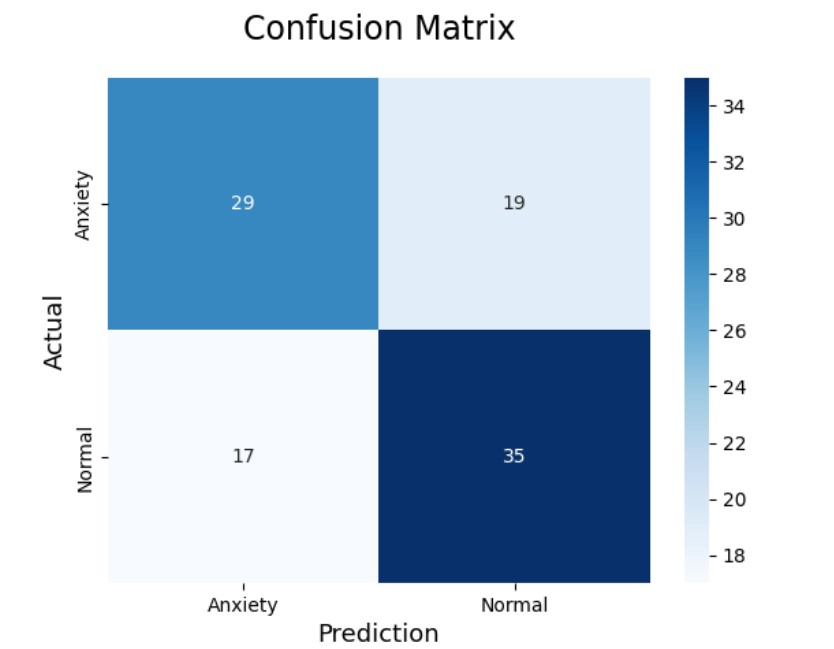
\includegraphics[width=0.8\textwidth]{Anxiety-Data-SmallData.jpg} % Replace with actual image path
\end{center}

\vspace{0.5cm} % Add 1 cm of vertical space (adjust as needed)

\subsubsection{Depression Data}
We used a dataset of 500 rows (small data).
\begin{itemize}
    \item \textbf{Hyperparameters:} ID, Text, Target
    \item \textbf{Target:} Normal (249), Depression (251)
    \item \textbf{Models:} Support Vector Classification (Support Vector Machine) with encoding Word2Vec
    \item \textbf{Results:}
    \begin{itemize}
        \item \textbf{Accuracy:} 0.62
        \item \textbf{Precision (average):} 0.6182
        \item \textbf{Precision for Depression Class:} 0.6182
        \item \textbf{Precision for Normal Class:} 0.6222
        \item \textbf{Recall:} 0.6667
        \item \textbf{Confusion Matrix:}
    \end{itemize}
\end{itemize}

\begin{center}
    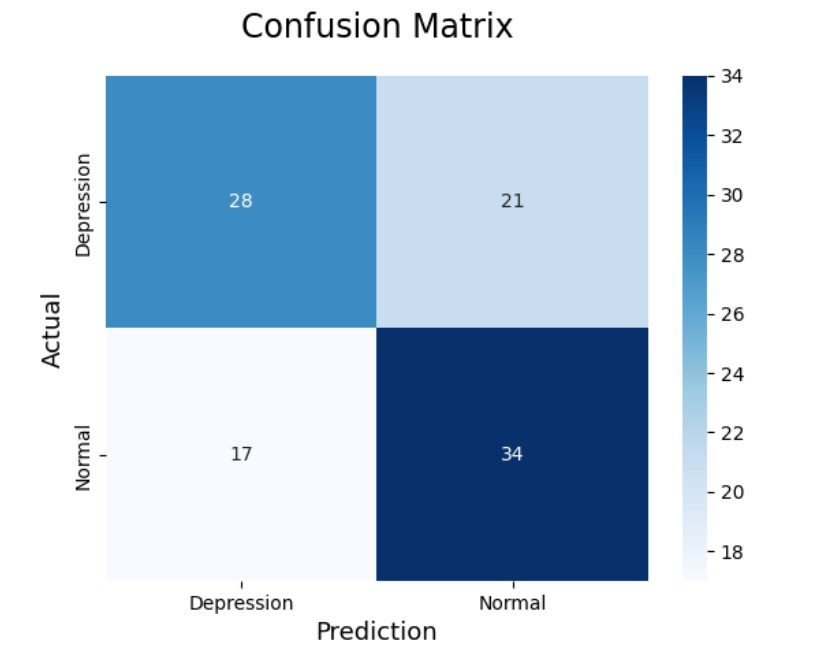
\includegraphics[width=0.8\textwidth]{Depression-Data-SmallData.jpg} % Replace with actual image path
\end{center}

\vspace{1cm} % Add 1 cm of vertical space (adjust as needed)

\subsection{Second Approach - Big Data}

\subsubsection{Anxiety Data - Linear Regression}

\begin{itemize}
    \item \textbf{Hyperparameters:} ID, Text, Target
    \item \textbf{Target:} Normal (246), Anxiety (254)
    \item \textbf{Models:} Support Vector Classification (Support Vector Machine) with encoding Word2Vec
    \item \textbf{Results:}
    \begin{itemize}
        \item \textbf{Accuracy:} 0.82
        \item \textbf{Average Precision:} 0.82
        \item \textbf{Precision for Anxiety Class:} 0.82
        \item \textbf{Precision for Normal Class:} 0.82
        \item \textbf{Recall for Anxiety Class:} 0.81
        \item \textbf{Recall for Normal Class:} 0.83
        \item \textbf{Confusion Matrix:}
    \end{itemize}
\end{itemize}

\begin{center}
    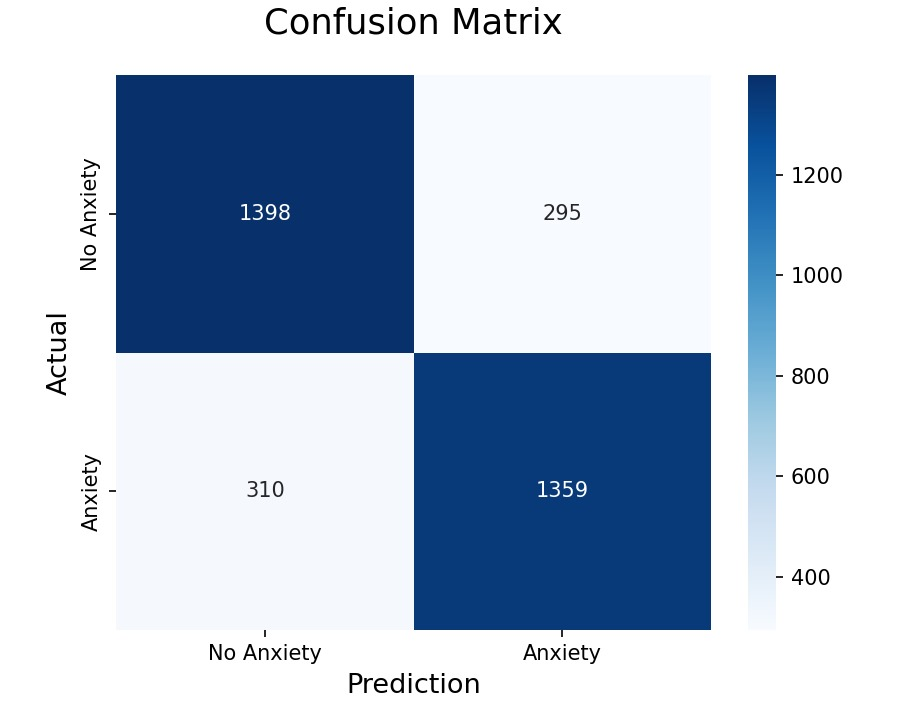
\includegraphics[width=0.8\textwidth]{Anxiety-Data-LinearRegression.jpg} % Replace with actual image path
\end{center}

\vspace{0.5cm} % Add 1 cm of vertical space (adjust as needed)

\subsubsection{Anxiety Data - Decision Tree}

\begin{itemize}
    \item \textbf{Hyperparameters:} ID, Text, Target
    \item \textbf{Target:} Normal (246), Anxiety (254)
    \item \textbf{Models:} Support Vector Classification (Support Vector Machine) with encoding Word2Vec
    \item \textbf{Results:}
    \begin{itemize}
        \item \textbf{Accuracy:} 0.83
        \item \textbf{Average Precision:} 0.83
        \item \textbf{Precision for Anxiety Class:} 0.88
        \item \textbf{Precision for Normal Class:} 0.79
        \item \textbf{Recall for Anxiety Class:} 0.75
        \item \textbf{Recall for Normal Class:} 0.90
        \item \textbf{Confusion Matrix:}
    \end{itemize}
\end{itemize}

\begin{center}
    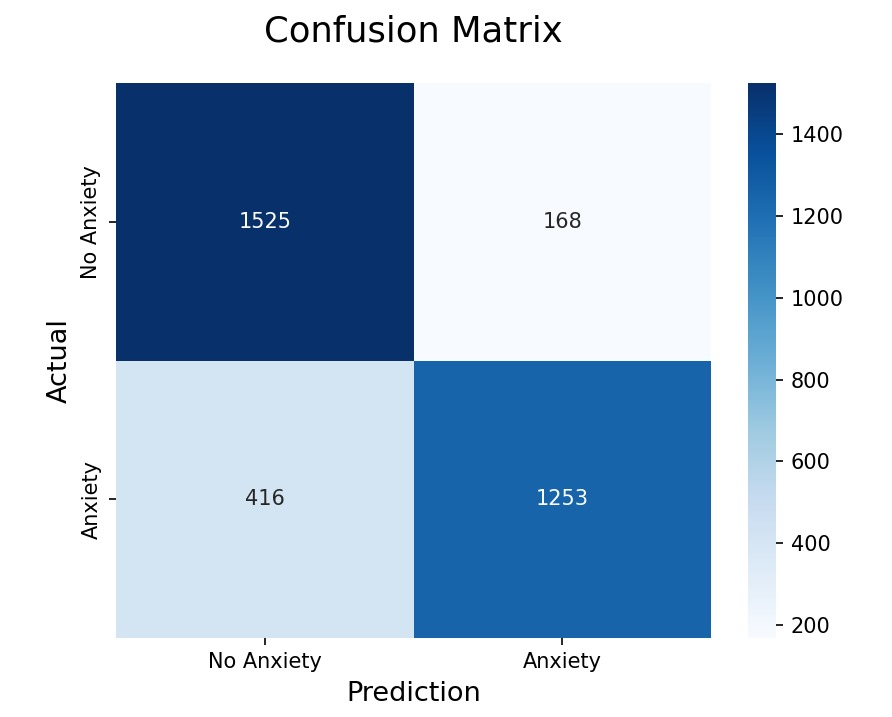
\includegraphics[width=0.8\textwidth]{Anxiety-Data-DecisionTree.jpg} % Replace with actual image path
\end{center}

\vspace{0.5cm} % Add 1 cm of vertical space (adjust as needed)

\subsubsection{Anxiety Data - Multi-layer Perceptron Classifier}

\begin{itemize}
    \item \textbf{Hyperparameters:} ID, Text, Target
    \item \textbf{Target:} Normal (246), Anxiety (254)
    \item \textbf{Models:} Support Vector Classification (Support Vector Machine) with encoding Word2Vec
    \item \textbf{Results:}
    \begin{itemize}
        \item \textbf{Accuracy:} 0.93
        \item \textbf{Average Precision:} 0.93
        \item \textbf{Precision for Anxiety Class:} 0.95
        \item \textbf{Precision for Normal Class:} 0.90
        \item \textbf{Recall for Anxiety Class:} 0.90
        \item \textbf{Recall for Normal Class:} 0.95
        \item \textbf{Confusion Matrix:}
    \end{itemize}
\end{itemize}

\begin{center}
    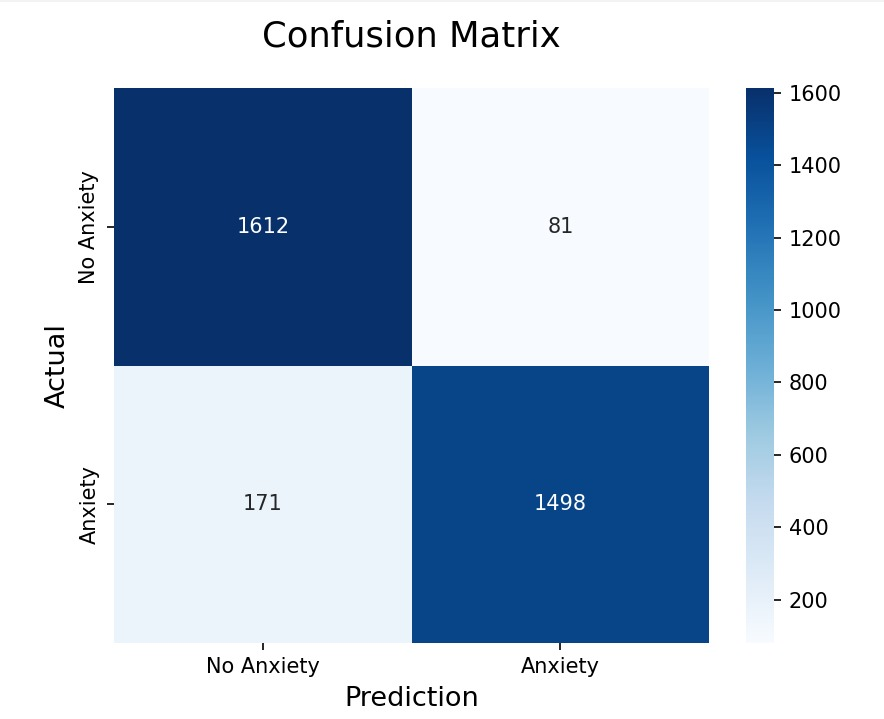
\includegraphics[width=0.8\textwidth]{Anxiety-Data-MLPClassifier.jpg} % Replace with actual image path
\end{center}

\vspace{0.5cm} % Add 1 cm of vertical space (adjust as needed)

\subsubsection{Depression Data - Linear Regression}
\begin{itemize}
    \item \textbf{Hyperparameters:} ID, Text, Target
    \item \textbf{Target:} Normal (249), Depression (251)
    \item \textbf{Models:} Support Vector Classification (Support Vector Machine) with encoding Word2Vec
    \item \textbf{Results:}
    \begin{itemize}
        \item \textbf{Accuracy:} 0.80
        \item \textbf{Average Precision:} 0.81
        \item \textbf{Precision for Depression Class:} 0.81
        \item \textbf{Precision for Normal Class:} 0.80
        \item \textbf{Recall for Depression Class:} 0.80
        \item \textbf{Recall for Normal Class:} 0.81
        \item \textbf{Confusion Matrix:}
    \end{itemize}
\end{itemize}

\begin{center}
    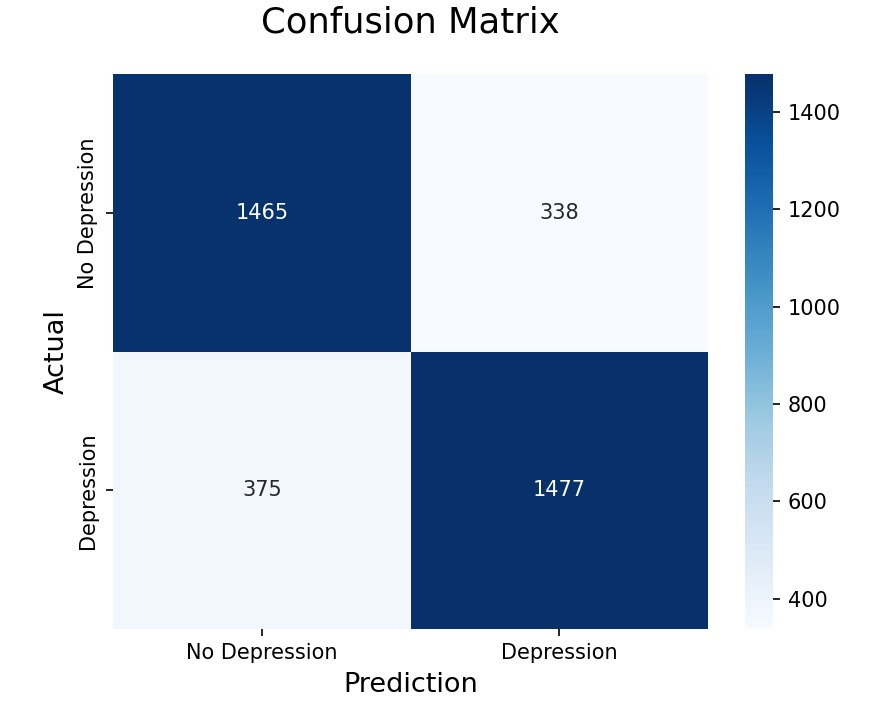
\includegraphics[width=0.8\textwidth]{Depression-Data-LinearRegression.jpg} % Replace with actual image path
\end{center}

\vspace{0.5cm} % Add 1 cm of vertical space (adjust as needed)

\subsubsection{Depression Data - Decision Tree}
\begin{itemize}
    \item \textbf{Hyperparameters:} ID, Text, Target
    \item \textbf{Target:} Normal (249), Depression (251)
    \item \textbf{Models:} Support Vector Classification (Support Vector Machine) with encoding Word2Vec
    \item \textbf{Results:}
    \begin{itemize}
        \item \textbf{Accuracy:} 0.83
        \item \textbf{Average Precision:} 0.84
        \item \textbf{Precision for Depression Class:} 0.89
        \item \textbf{Precision for Normal Class:} 0.78
        \item \textbf{Recall for Depression Class:} 0.75
        \item \textbf{Recall for Normal Class:} 0.91
        \item \textbf{Confusion Matrix:}
    \end{itemize}
\end{itemize}

\begin{center}
    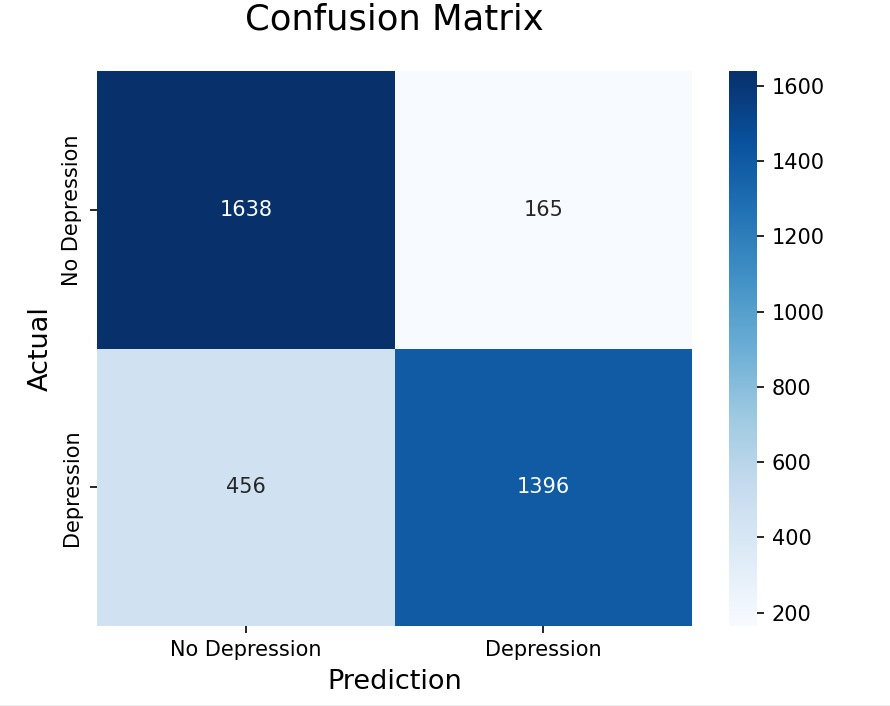
\includegraphics[width=0.8\textwidth]{Depression-Data-DecisionTree.jpg} % Replace with actual image path
\end{center}

\vspace{0.5cm} % Add 1 cm of vertical space (adjust as needed)

\subsubsection{Depression Data - Multi-layer Perceptron Classifier}
\begin{itemize}
    \item \textbf{Hyperparameters:} ID, Text, Target
    \item \textbf{Target:} Normal (249), Depression (251)
    \item \textbf{Models:} Support Vector Classification (Support Vector Machine) with encoding Word2Vec
    \item \textbf{Results:}
    \begin{itemize}
        \item \textbf{Accuracy:} 0.93
        \item \textbf{Average Precision:} 0.93
        \item \textbf{Precision for Depression Class:} 0.96
        \item \textbf{Precision for Normal Class:} 0.90
        \item \textbf{Recall for Depression Class:} 0.89
        \item \textbf{Recall for Normal Class:} 0.97
        \item \textbf{Confusion Matrix:}
    \end{itemize}
\end{itemize}

\begin{center}
    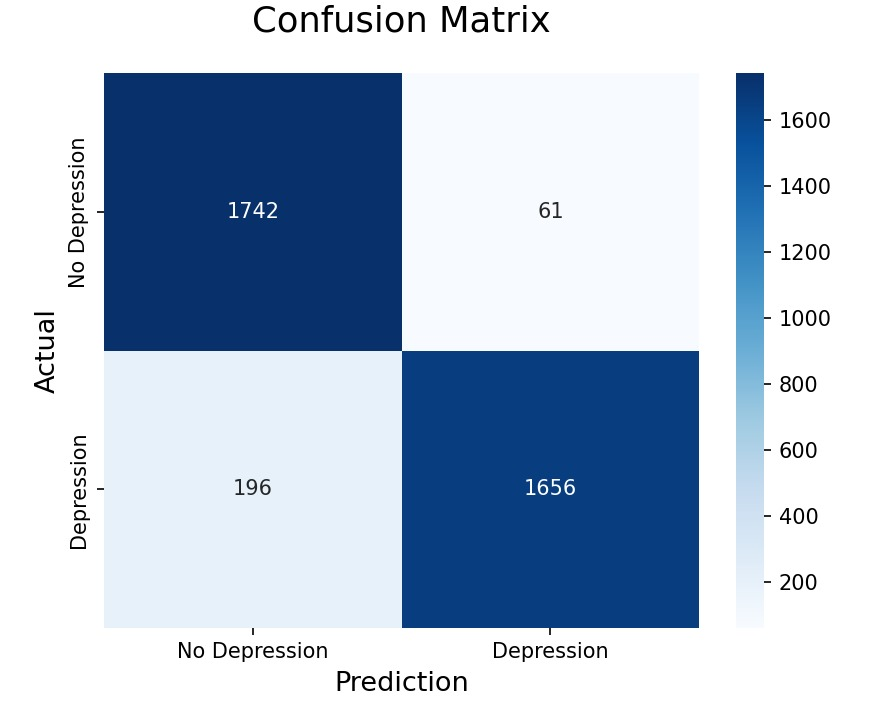
\includegraphics[width=0.8\textwidth]{Depression-Data-MLPClassifier.jpg} % Replace with actual image path
\end{center}

\end{document}
